\documentclass[11pt]{article}
\usepackage[sc]{mathpazo} 
\usepackage{fullpage}
\usepackage{natbib}
\linespread{1.7}
\usepackage[utf8]{inputenc}
\usepackage{lineno}
\usepackage{titlesec}
\titleformat{\section}[block]{\Large\bfseries\filcenter}{\thesection}{1em}{}
\titleformat{\subsection}[block]{\Large\itshape\filcenter}{\thesubsection}{1em}{}
\titleformat{\subsubsection}[block]{\large\itshape}{\thesubsubsection}{1em}{}
\titleformat{\paragraph}[runin]{\itshape}{\theparagraph}{1em}{}[. ]\renewcommand{\refname}{Literature Cited}
% my addnl packages
\usepackage{geometry}
\usepackage{graphicx}
\usepackage[T1]{fontenc}
\usepackage{authblk}
\usepackage{setspace}
\usepackage{amsfonts,amssymb,amsmath,hyperref}
\usepackage{float}
\usepackage{caption}
\usepackage{multirow}
\usepackage{hyperref}
\usepackage{wrapfig}
\usepackage{rotating}
\usepackage[usenames,dvipsnames]{xcolor}
\newcommand{\revise}[1]{{\color{Mahogany}{#1}}}
\usepackage[normalem]{ulem}
\graphicspath{{/Users/jm200/Library/CloudStorage/Dropbox/Miller Lab/github/POAR-Forecasting/Manuscript/Figures/}}
\newcommand{\tom}[2]{{\color{red}{#1}}\footnote{\textit{\color{red}{#2}}}}


\doublespacing


%-------------------------------------------------------------------------
\title{Using matrix projection model to predict climate-induced range expansion/contraction for a dioecious range-limited species}

\author[1]{Jacob K. Moutouama}
\author[2]{Aldo Compagnoni}
\author[1]{Tom E.X. Miller}
\affil[1]{Program in Ecology and Evolutionary Biology, Department of BioSciences, Rice University, Houston, TX USA}
\affil[2]{Institute of Biology, Martin Luther University Halle-Wittenberg, Halle, Germany; and German Centre for Integrative Biodiversity Research (iDiv), Leipzig, Germany}
%-------------------------------------------------------------------------
\usepackage{Sweave}
\begin{document}
%\SweaveOpts{concordance=TRUE}
\maketitle
\noindent{} $\ast$ Corresponding author: jmoutouama@gmail.com\\
\noindent{} Submitted to \textit{Ecological Monographs}\\
\noindent{} Manuscript type: Article\\
\noindent{} Open Research statement: All of our data and code are available during peer review at \url{https://github.com/jmoutouama/POAR-Forecasting}. This manuscript and its contents can be reproduced from this file: \url{https://github.com/jmoutouama/POAR-Forecasting/Manuscript/Forescasting.Rnw}. All data are provided at \url{https://github.com/jmoutouama/POAR-Forecasting/tree/main/data}.
%\SweaveOpts{concordance=TRUE}

\linenumbers
%-------------------------------------------------------------------------
\newpage
\section*{Abstract}

% Sex-specific response to rising temperature and drought raises the questions of whether global change could lead to a drastic change in the sex ratio and whether that change in the sex ratio could drive population extinction or population range shift.
% Answering these questions requires an understanding of the mechanism by which a change in vital rates under future climate conditions for both male and female, could be translated into a significant change in population dynamics.
% The geographic ranges of most species are limited by climatic factors, including temperature and precipitation. 
% Any change in the magnitude of these factors in a given location will impact the organisms that live there. 
% Females and males tend to respond differently to climate change.
% This sex-specific response to climate change could have implications on range shift (warmer climate leading to species moving to cooler locations). 
% Although the response to warming is generally understood, it is difficult to disentangle the interaction between sex and climate drivers to understand their relative contribution and effects on population dynamics and the consequence of such effect on range shift. 
% Disentangle the relative effect of sex ratio and climate drivers on population fitness and the implications of such  effect on species range shift is crucial step toward building forecast models for dioecious plants. 
% Here, we built a forecast model for dioecious plants by understanding sex-specific demographic responses to climate change.
% Combining a demographic data set for a dioecious species with a Bayesian hierarchical modeling approach, we fit models in which vital rates are driven by precipitation and temperature of the growing season.
% We developed a forecasting model using hierarchical Bayesian matrix models for Texas bluegrass (Poa arachnifera) to project its potential range shifts in response to climate change. 


%-------------------------------------------------------------------------
\section*{Keywords}
% climate change, demography, forecasting, matrix projection model, mechanistic models, sex ratio, range limits

%--------------------------------------------------------------------
\newpage
\section*{Introduction}
Rising temperatures and extreme drought events associated with global climate change are leading to increased concern about how species will become redistributed across the globe under future climate conditions \citep{bertrand2011changes,gamelon2017interactions}.
Dioecious species might be particularly vulnerable to the influence of climate change because they often display skewed sex ratios that are generated or reinforced by sexual niche differentiation (distinct responses of females and males to shared climate drivers) \citep{Tognetti2012}. 
Accounting for such a niche differentiation between male and female within a population is a long-standing challenge in accurately predicting which sex will successfully track environmental change and how this will impact population dynamics \citep{jones1999sex,gissi2023exploring}. 
The vast majority of theory and models in population biology, including those used to forecast biodiversity responses to climate change, ignore the complication of sex structure \citep{pottier2021sexual,ellis2017does}.
As a result, accurate forecasts of colonization-extinction dynamics for dioecious species under future climate scenarios are limited. 

Females and males respond differently to climate change, especially in species where the two sexes have different energetic requirements or habitat preferences \citep{gissi2023exploring,gissi2023sex,hultine2016climate}. 
This sex-specific response to climate change may help one sex to succeed in extreme climatic conditions rather than the other sex \citep{zhao2012sex, burli2022environmental}.
Experimentation manipulation revealed that when exposed to increasing temperatures, for example, in two populations of Atlantic marine copepods (\textit{Acartia tonsa}), males showed significantly lower survival than females \citep{sasaki2019complex}. 
In some species, such as the Asutralian flying fox or Populus cathayana, females showed lower survival than males in response to extreme temperature \citep{welbergen2008climate,zhao2012sex}.
Therefore, in the context of climate, populations in which males are rare could experience low reproductive success due to sperm or pollen limitation that may lead to population decline \citep{eberhart2017sex}.

The geographic range of most species is limited by climatic factors, including temperature, precipitation. 
Any shift in the magnitude of these climatic factors in a given location will impact the population viability, with potential implication on range shift \citep{davis2001range, pease1989model}. 
This is particularly true for dioecious species.
For instance, in \textit{Valeriana edulis} populations, a reduction in water availability due to climate change implies that male valarians are likely to move upslope, which reduces pollen limitation, increases seedset and favor range expansion \citep{petry2016sex}.
Although the response to warming is generally understood, it is difficult to disentangle the interaction between sex and climate drivers to understand their relative contribution and effects on population dynamics and the consequence of such population dynamics on range dynamic. 

Our ability to track the impact of climate change on the population dynamics of dioecious plants and the implication of such impact on range shift depends on our ability to build mechanistic models that take into account the spatial and temporal context in which sex specific response to climate change affects population viability \citep{davis2001range,evans2016towards,czachura2020demographic}.
At their range edge where climatic conditions are expected to be less favorable, if dioecious species populations are non-viable in response to climate change, global warming will induce range contraction in dioecious species.
In reverse, if populations at the edge are viable habitats in response to global warming, dioecious species populations could shift their range and relocate to more favorable and thereby favored range expansion. 

In this study, we used a mechanistic approach by combining common field experiment and matrix projection modelling, to understand the demographic response of dioecious species to climate change and its implications for future range dynamics.
Our study system is a dioecious plant species (\textit{Poa arachnifera}) distributed along environmental gradients in the south-central US corresponding to variation in temperature across latitude and precipitation across longitude (MAP). 
% A previous study showed that, despite the differentiation of the climatic niche between sexes, the female niche mattered the most in driving the environmental limits of population viability \citep{miller2022two}. 
Here, we asked three questions: (1) What is the sex-specific demographic response to rising temperature and precipitation ?
(2) How that sex-specific demographic response affects populations dynamics under current and future climatic conditions ?
(3) What are the implications of population dynamics on range dynamics ?   

%--------------------------------------------------------------------
\section*{Materials and methods}

\subsection*{Study species}
Texas bluegrass (\textit{Poa arachnifera}) is a perennial, summer-dormant cool-season (C3) grass. 
The species occurs in Texas, Oklahoma, and southern Kansas, USA \citep{hitchcock1971manual}. 
Texas bluegrass grows during cool months between October and May, with onset of dormancy often from June to September \citep{kindiger2004interspecific}.
Flowering occurs in May and the species is pollinated by wind \citep{hitchcock1971manual}.

\subsection*{Common garden experiment}

We set up a common garden experiment to manipulate climatic factors such as temperature and precipitation to detect mechanisms underlying sex-specific demographic response to climate and the implication of such a response on range limitation \citep{merow2017climate,schwinning2022common}. 
At this end, we collected vegetative tillers from flowering individuals of each sex in eight natural (sources) populations of the focal species.
We then propagated these tillers in ProMix plotting soil and supplemented them with Osmocote slow-release fertilizer at $75^\circ$F to $85^\circ$F under natural climatic conditions at the Rice University Greenhouse. 
The common experiment was installed on 14 sites across a precipitation gradient (FigX). At each site, we established 14 blocks. Each block was selected so that they resemble the natural environment of the species. For each block we planted three females and three males individuals. We spared the individuals, provided \~ 1 L  of water, and removed surrounding vegetation to avoid competition and promote establishment. 


\subsection*{Demographic and climatic data collection}
In each site we collected individual demographic data including survival, growth (number of tillers), flowers and fertility (number of panicle) for two censuses (2015 and 2016) to build our demographic models.
\tom{The details of the data collection has been provided in \cite{miller2022two}.}{You need to say a little more here.} 

We want to understand how current and future climate affect the \tom{dynamic}{This is vague. This carefully about the target of your analysis and the best way to describe it.} of \textit{Poa arachnifera}. 
Therefore, we considered the climatic data from the time we collected demographic data \tom{(2015 and 2016 censuses)}{The timeline of the experiment and the censuses need to be clarified. Above you say 2014-15 and here you say 2015-16.} \tom{as the current condition for the species}{Unclear what this means.}.
\tom{Additionally, months were aligned to match demographic transition years rather than calendar years.}{Needs to be explained.}
Monthly temperature and precipitation data were downloaded for each site from Chelsea \citep{karger2017climatologies}. 
We define June to September as the dormant season of the year and the rest of the year as the growing season. 
\tom{We used seasonal data because they allowed us to quantify the response of species to change in seasonal change in climate.}{This sentence contains no information.} 
\tom{We evaluated future climate projections from two scenarios}{I suggest that you first introduce the model and its parameterization with current climate data, and then describe the climate projections in a later section of the methods.}: SSP 370, an intermediate-to-pessimistic scenario assuming a radiative forcing to amount to 7.0 $W m^{-2}$ by 2100, and SSP 585, a pessimistic emission scenario which project a radiative forcing to amount to 8.5 $W m^{-2}$ by 2100 \citep{o2017roads,brun2022global}.
\tom{The precipitation of growing season and dormant season were not explained by the Temperature of growing season and dormant season \textcolor{blue}{(Appendix S1: Figure S1)}.}{Explain why this is significant and why you looked for this.}

\subsection*{Sex ratio experiment}
\tom{We}{I would describe the demographic data before the sex ratio experiment.} also conducted a sex-ratio experiment to measure the effect of male panicle availability on seed viability on females panicles. 
\tom{Details of the experiment are provided in \cite{compagnoni2017can} and \cite{miller2022two}. }{Again, you need more info here.}

We used the sex-ratio to estimate the probability of viability and the germination rate. 
Seed viability was modeled with a binomial distribution where the probability of viability ($v$) was given by:
\begin{align}\label{eq:viab_fn}
v = v_{0} * (1 - OSR^{\alpha})
\end{align}

\noindent {where $OSR$ is the \tom{operational sex ratio}{This concept should be descibed in the Introduction.} (proportion of panicles that were female) in the experimental populations.
The properties of the above function is supported by our previous work \citep{compagnoni2017can}. 
Here, seed viability is maximized at $v_{0}$ as $OSR$ approaches zero (strongly male-biased) and goes to zero as $OSR$ approaches $1$ (strongly female-biased).
Parameter $\alpha$ controls how viability declines with increasing female bias.

We used a binomial distribution to model the germination data from greenhouse trials.
Given that germination was conditional on seed viability,the probability of success was given by the product $v*g$, where $v$ is a function of $OSR$ (Eq. \ref{eq:viab_fn}) and $g$ is assumed to be constant.

\subsection*{Vital rate responses to climate}
We used individual level measurements of survival, growth (number of tillers), flowering, number of panicles to independently develop Bayesian mixed effect models describing how each vital rate varies as a function of sex, size, precipitation of growing and dormant season and temperature of of growing and dormant season. 
We fit two versions of the vital rate models, with either linear or second-degree polynomial functions for the influence of climate, and used model selection to quantify their empirical support.
We included a second-degree polynomial because we expected that climate variables would affect vital rates through a hump-shaped relationship. 

We centered and standardized all predictors to facilitate model convergence.
We included site, \tom{source, and block}{You have not described these.} as random effect.
All the vital rate models used the same \tom{linear and quadratic predictor}{show these} for the expected value ($\mu$). 
However, we applied a different link function ($f(\mu)$) depending on the distribution the vital rate \textcolor{blue}{(Appendix S1: Section S1)}. 
We modeled survival and flowering data with a Bernoulli distribution.
We modeled the growth (tiller number) with a zero-truncated Poisson inverse Gaussian distribution. 
Fertility (panicle count) was model as zero-truncated negative binomial. 
We fit all models in Stan \citep{rstan}, with weakly informative priors for coefficients ($\mu = 0, \sigma = 100$) and variances ($\gamma [0.001, 0.001]$). We ran three chains for 1000 samples for warmup and 40000 for interactions, with a thinning rate of 3.
We accessed the quality of the models using trace plots and predictive check graphs \citep{piironen2017comparison} \textcolor{blue}{(Appendix S1: Figure S1)}.
Then, we used approximate Bayesian leave-one-out cross-validation (LOOIC) to select the best model describing the effect of climate variable on vital rate. The final model was the model with the lowest LOOIC \citep{vehtari2017practical}. 

\tom{To understand the effect of climate on vital rates, we used the 95 \% credible interval of the final model for each vital rate. When the 95 \% credible interval of the coefficient of a given climatic variable did not include zero, we concluded that there is a strong effect of that variable on the vital rate. 
In contrast, when we have a credible interval of a climatic variable that includes zero, we used the empirical cumulative distribution to find the probability that the coefficient of that climatic variable is greater than zero.}{I would prefer to not interpret the coefficient posteriors in this way, because it is effectively frequentist hypothesis-testing.}


\subsection*{Population growth rate responses to climate}
To understand the effect of climate on population growth rate, we used the vital rate estimated earlier to build a matrix projection model (MPM) structured by size (number of tillers) and sex with \tom{"Climate"}{why quotes?} as covariate.  
\tom{For a given climatic variable}{I am not sure why this is conditional on a climate variable. I think you are suggesting that this model applies to a specific level of climate values. However, I think you should instead modify the notation of the model so that it is explicitly climate-dependent, eg $F_{x,c,t}$}, let $F_{x,t}$ and $M_{x,t}$ be the number of female and male plants of size $x$ in year $t$, where $x \in \{1,2,...,U\}$ and $U$ is the maximum number of tillers a plant can reach (here 99th percentile of observed maximum size). 
Let $F^{R}_{t}$ and $M^{R}_{t}$ be the new recruits, which we assume do not reproduce in their first year.
We assume that the parameters of sex ratio-dependent mating (Eq. \ref{eq:viab_fn}) do not vary with climate.  
For a pre-breeding census, the expected numbers of recruits in year $t+1$ is given by:
\begin{align}\label{eq:recruits}
F^{R}_{t+1} = \sum_{x=1}^{U} 	[ \, p^{F}(x) \cdot c^{F}(x) \cdot d \cdot v(\mathbf{F_{t}},\mathbf{M_{t}}) \cdot m \cdot \rho 	] \, F_{x,t}
\\
M^{R}_{t+1} = \sum_{x=1}^{U} 	[ \, p^{F}(x) \cdot c^{F}(x) \cdot d \cdot v(\mathbf{F_{t}},\mathbf{M_{t}}) \cdot m \cdot (1-\rho) 	] \, F_{x,t}
\end{align}

\noindent where $p^{F}$ and $c^{F}$ are flowering probability and panicle production for females of size $x$, $d$ is the number of seeds per female panicle, $v$ is the probability that a seed is fertilized, $m$ is the probability that a fertilized seed germinates, and $\rho$ is the primary sex ratio (proportion of recruits that are female). 
Seed fertilization depends on the OSR of panicles (following Eq. \ref{eq:viab_fn}) which was derived from the $U \times 1$ vectors of population structure $\mathbf{F_{t}}$ and $\mathbf{M_{t}}$:
\begin{align}\label{eq:viab_MPM}
v(\mathbf{F_{t}},\mathbf{M_{t}}) = v_{0} * \left[ 1 - \left( \frac{\sum_{x=1}^{U} p^{F}(x) c^{F}(x) F_{x,t}}{\sum_{x=1}^{U} p^{F}(x) c^{F}(x) F_{x,t} + p^{M}(x) c^{M}(x) M_{x,t}} \right) ^{\alpha}\right]
\end{align}

Thus, the dynamics of the size-structured component of the population are given by:
\begin{align}\label{eq:dynamics}
F_{y,t+1} = [ \, \sigma \cdot g^{F}(y,x=1) ] \, F^{R}_{t} + \sum_{x=1}^{U} 	[ \, s^{F}(x) \cdot g^{F}(y,x)] \, F_{x,t}
\\
M_{y,t+1} = [ \, \sigma \cdot g^{M}(y,x=1) ] \, M^{R}_{t} + \sum_{x=1}^{U} 	[ \,  s^{M}(x) \cdot g^{M}(y,x) ] \, M_{x,t}
\end{align}

\noindent In the two formula above, the first term represents seedlings that survived their first year and enter the size distribution of established plants.
Instead of using \textit{P. arachnifera} survival probability, we used the seedling survival probability ($\sigma$) from demographic studies of the hermaphroditic congener \textit{Poa autumnalis} in east Texas (T.E.X. Miller and J.A. Rudgers, \textit{unpublished data}), and we assume this probability was constant across sexes and climatic variables. 
We did this because we had little information on the early life cycle transitions of \tom{greenhouse-raised transplants}{You have not described these.}. 
We also assume that $g(y,x=1)$ is the probability that a surviving seedlings reach size $y$, the expected future size of 1-tiller plants from the transplant experiment.
The second term represents survival and size transition of established plants from the previous year, where $s$ and $g$ give the probabilities of surviving at size $x$ and growing from sizes $x$ to $y$, respectively, and superscripts indicate that these functions may be unique to females ($F$) and males ($M$).

Because the two-sex MPM is nonlinear (vital rates affect and are affected by population structure) we estimated the asymptotic geometric growth rate ($\lambda$) by numerical simulation, and repeated this across a range of climate.

\subsection*{Identifying the mechanisms of population growth rate sensitivity to climate }
\tom{}{I don't think the LTRE analysis is adequately motivated by the Intro.}
To identify the mechanism by which climate affects population growth rate, we decomposed the effect of each climate variable (here Climate) on population growth rate ($\lambda$) into contribution arising from the effect on each stage-specific vital rate \citep{caswell2000matrix}.
At this end we used a life table response experiment (LTRE) with a regression designs. 
The LTRE approximates the change in $\lambda$ with climate  as the product of the sensitivity of $\lambda$ to the parameters times the sensitivity of the parameters to climate, summed over all parameters \citep{caswell1989analysis}:
\begin{align}\label{eq:ltre}
\frac{\partial \lambda}{\partial Climate} \approx \sum_{i} \frac{\partial \lambda}{\partial \theta^{F}_{i}} \frac{\partial \theta^{F}_{i}}{\partial Climate} + \frac{\partial \lambda}{\partial \theta^{M}_{i}} \frac{\partial \theta^{M}_{i}}{\partial Climate}
\end{align}

\noindent where, $\theta^{F}_{i}$ and $\theta^{M}_{i}$ represent sex-specific parameters: the regression coefficients for the intercepts and slopes of size-dependent vital rate functions. 
Because LTRE contributions are additive, we summed across vital rates to compare the total contributions of female and male parameters. 

\subsection*{Implication on niche breath and range expansion/contraction}
To understand the implication of our study on \tom{niche breath}{You have not defined this, or described how it relates to geographic ranges.}, we projected the population growth current and future prediction on two axes of climatic conditions (temperature and precipitation) of each seasonal season (dormant and growing season). 
Similarly, to understand the implication of our study on range contraction on expansion, we extrapolate population growth current and future prediction across the range to map species distributions. 

All the analysis were performed in R 4.3.1 \citep{RCoreteam}


\section*{Appendix S1}
\renewcommand{\thefigure}{S\arabic{figure}}
	\setcounter{figure}{0}
	
		\renewcommand{\thetable}{S\arabic{table}}
	\setcounter{equation}{0}  % reset counter 
	\setcounter{figure}{0}
	\setcounter{table}{0}
	
	
	\begin{figure}[H]
		\centering
		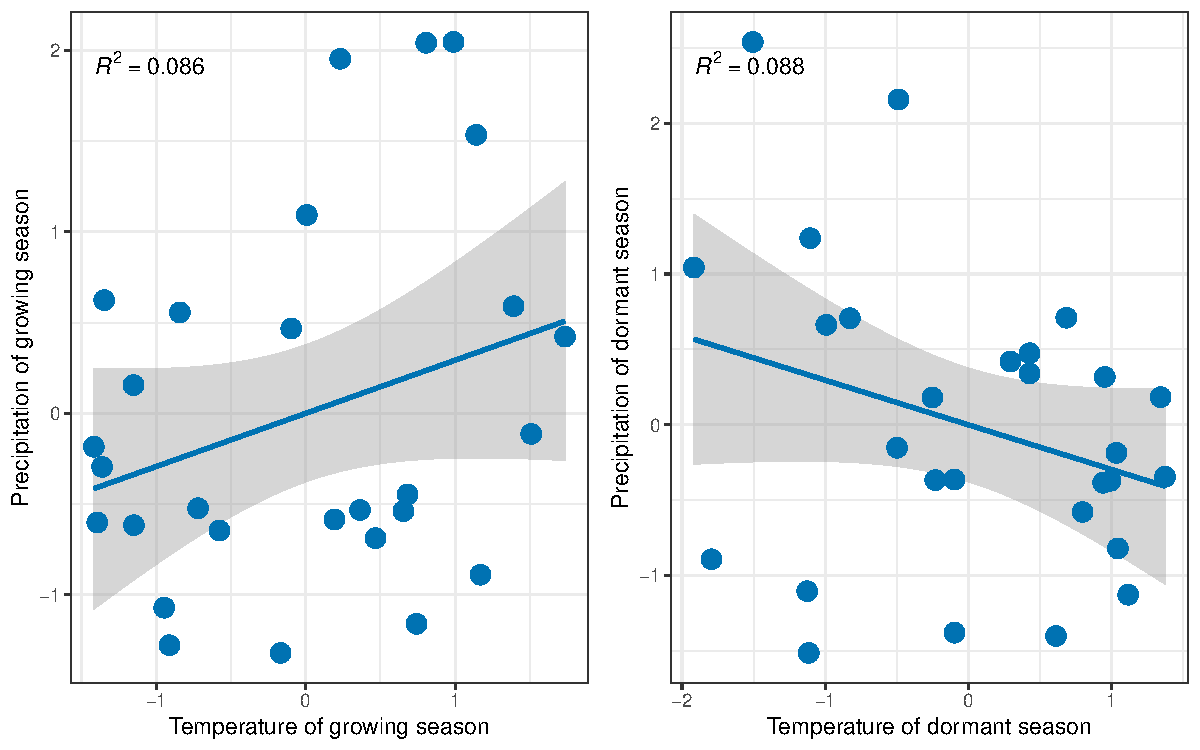
\includegraphics[width = \linewidth]{Figures/Varianceexplained.pdf}
		\caption{\textbf{Relation between precipitation and temperature for each season (growing and dormant).} $R^2$ indicates the value of proportion of explained variance between the temperature and precipitation}
	\end{figure}
	
  \begin{figure}[H]
		\centering
		\includegraphics[width = \linewidth]{Figures/PPC.pdf}
		\caption{\textbf{Consistency between real data and simulated values suggests that the fitted model accurately describes the data}. Graph shows density curves for the observed data (light blue ) along with the simulated values (dark blue). The first column shows the linear models and the second column shows the 2 degree polynomial models.}
	\end{figure}

\subsection*{Section S1}
\begin{subequations} 
	\begin{align}
		   S \sim Bernoulli(\hat{S}) \\
		   F \sim Bernoulli(\hat{F}) \\
		   G \sim Zero-truncated \ Poisson \ inverse\ Gaussian(\hat{G}) \\
		   Fer \sim Zero-truncated \ negative \ binomial(\hat{Fer}) 
    \end{align}
\end{subequations}
\begin{subequations} 
	\begin{align}
		   \hat{S} = \frac{exp (f(\mu))}{1 + exp (f(\mu))}  \\
		   \hat{F} = \frac{exp (f(\mu))}{1 + exp (f(\mu))}  \\
		   \textcolor{red}{\hat{G} = exp (f(\mu))} \\
		   \textcolor{red}{\hat{Fer} = exp (f(\mu))}
    \end{align}
\end{subequations}
\begin{equation} \label{eq:f_rate}
\begin{split}
f(\mu) = \beta_{0} + \beta_{1}size + \beta_{2}sex + \beta_{3}pptgrow + \beta_{4}pptdorm + \beta_{5}tempgrow\\ 
+ \beta_{6}tempdorm + \beta_{7}pptgrow*sex + \beta_{8}pptdorm*sex + \beta_{9}tempgrow*sex \\ 
+ \beta_{10}tempdorm*sex + \beta_{11}size*sex + \beta_{12}pptgrow*tempgrow\\
+ \beta_{13}pptdorm*tempdorm + \beta_{14}pptgrow*tempgrow*sex\\
+ \beta_{15}pptdorm*tempdorm*sex + \beta_{16}pptgrow^2 + \beta_{17}pptdorm^2 \\
+ \beta_{18}tempgrow^2 + \beta_{19}tempdorm^2 + \beta_{20}pptgrow^2*sex \\
+ \beta_{21}pptdorm^2*sex + \beta_{22}tempgrow^2*sex \\ 
+ \beta_{23}tempdorm^2*sex + \phi + \rho + \nu 
\end{split}
\end{equation}

\bibliographystyle{ecology}
\bibliography{Forecasting}
\end{document}
